\documentclass[../main.tex]{subfiles}

\begin{document}
    \section{Tujuan}
        Tujuan dari praktikum ini sebagai berikut,
        \begin{enumerate}
            \item Memahami proses konversi representasi state space ke bentuk representasi fungsi alih
            \item Memahami proses identifikasi sistem dengan perangkat lunak MATLAB
        \end{enumerate}
        dst ....................................................
        
    \section{Dasar Teori}
        Representasi \textit{state space} dapat digunakan untuk mempresentasikan sistem MIMO (\textit{Multi Input Multi Output}). Sistem MIMO memiliki jumlah fungsi transfer sistem sama dengan jumlah kombinasi dari input dan outputnya. Dalam pengujian sistem secara langsung, banyak sistem yang tidak diketahui parameter dan karakteristiknya. Oleh karena itu, dibutuhkan cara untuk mengidentifikasi parameter sistem serta mempelajari karakteristik sistem dari representasi model sistem. Identifikasi terbagi atas dua jenis yaitu, \textit{black box modelling} dan \textit{grey box modelling}. \textit{black box modelling} merupakan metode identifikasi sistem yang hanya diketahui nilai \textit{input} dan nilai \textit{output} sistem saja. \textit{grey box modelling} merupakan pemodelan sistem yang mencari parameter dari sistem yang telah diketahui model matematisnya \cite{fmz2023attitude,fmz2023trajectory}.
        
        dst ....................................................
        
        
    \section{Hasil dan Pembahasan}
        \subsection{Pemodelan Motor DC}
            \subsubsection{Pemodelan state space}
                \begin{figure}[H]
                    \centering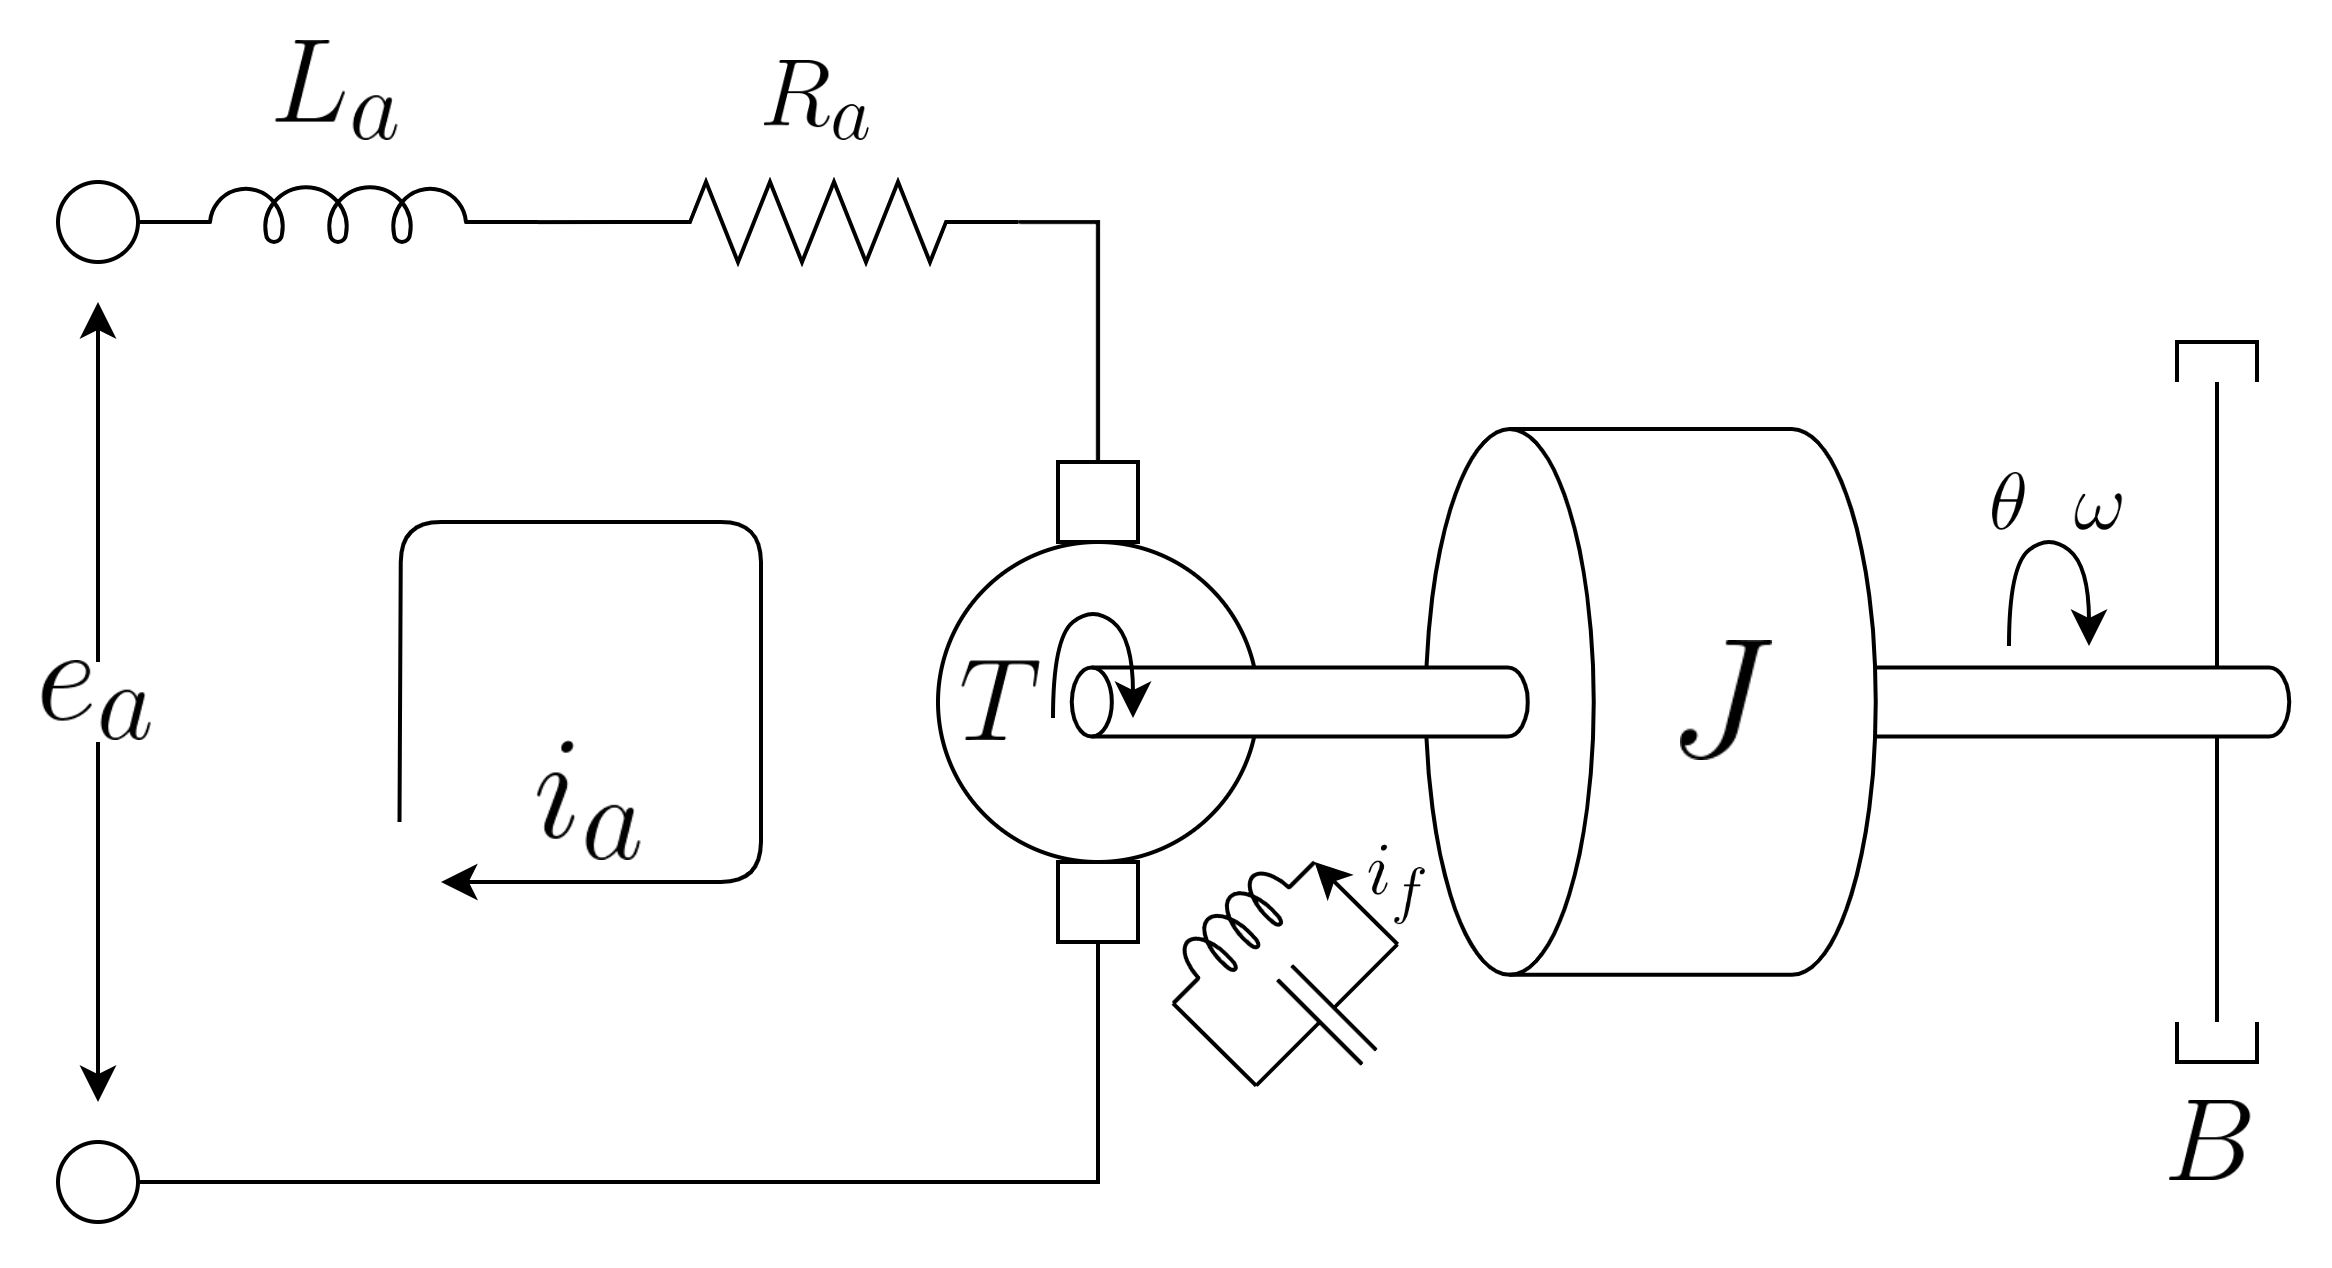
\includegraphics[width = 0.7\textwidth]{assets/image/pemodelan_motor.png}
                    \caption{Sistem Model Elektrik dan Mekanik Motor DC}
                    \label{gambar_1}
                \end{figure}
                Persamaan rangkaian elektrik pada motor dapat dianalisa dengan hukum kirchoff sebagai berikut,
                \begin{equation}
                    \begin{split}
                        e_a - e_{ggl} &= L_a\frac{di_a}{dt} + R_a i_a \\[5pt]
                        e_a &= L_a \frac{di_a}{dt} + R_a i_a + e_{ggl}
                    \end{split}
                \end{equation}
                \begin{equation}
                    \begin{split}
                        e_{ggl} &= K_m i_f \frac{d\theta}{dt} \\[5pt]
                        e_{ggl} &= K_m \frac{d\theta}{dt}
                    \end{split}
                \end{equation}
                \begin{equation}
                    \begin{split}
                        e_a &= L_a\frac{di_a}{dt} + R_a i_a + K_m\frac{d\theta}{dt} \\[5pt]
                        L_a\frac{di_a}{dt} &= -K_m\frac{d\theta}{dt} - R_a i_a + e_a \\[5pt]
                        \frac{di_a}{dt} &= -\frac{K_m}{L_a}\frac{d\theta}{dt} - \frac{R_a}{L_a}i_a + \frac{1}{L_a}e_a \\[5pt]
                        \dot{i_a} &= -\frac{K_m}{L_a}\dot{\theta} - \frac{R_a}{L_a}i_a + \frac{1}{L_a}e_a
                    \end{split}
                \end{equation}
                
                dst ....................................................
               
            \subsubsection{Generate data dari pemodelan untuk identifikasi}
                Hasil pemodelan fungsi alih dimasukkan ke simulink untuk menghasilkan data input dan output sebagai berikut,
                \begin{figure}[H]
                    \centering
                    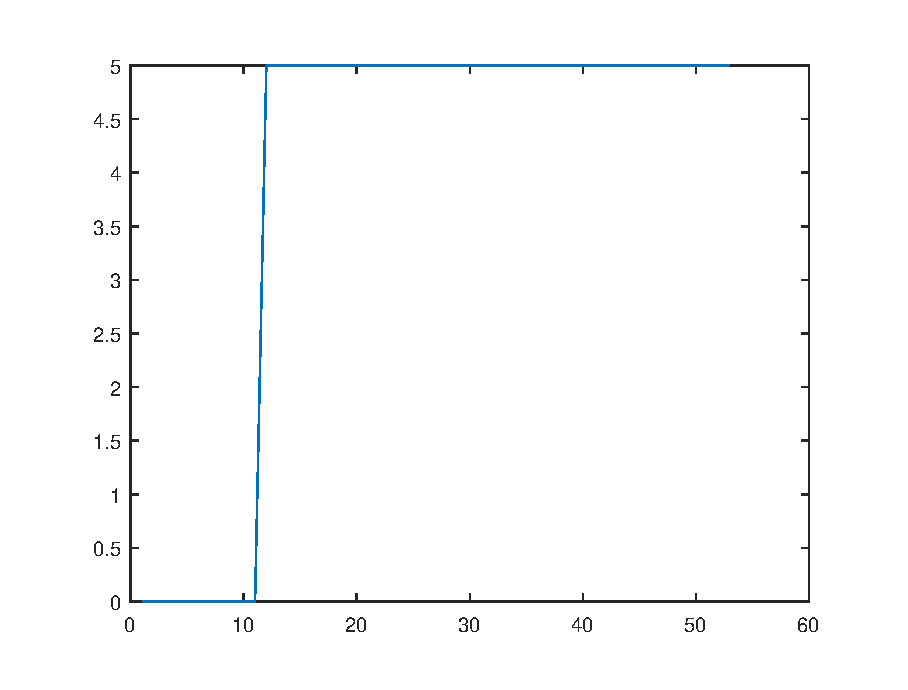
\includegraphics[width = 0.7\textwidth]{assets/image/INPUT.eps}
                    \caption{Data input berupa sinyal step}
                    \label{gambar_2}
                \end{figure}
                \begin{figure}[H]
                    \centering
                    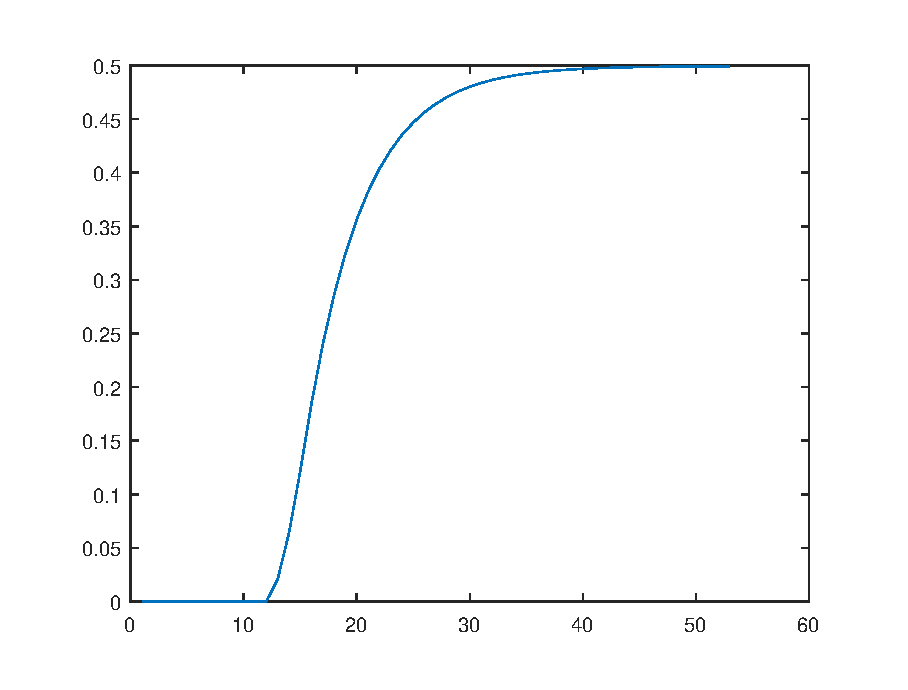
\includegraphics[width = 0.7\textwidth]{assets/image/OUTPUT.eps}
                    \caption{Data output berupa respon sistem}
                    \label{gambar_3}
                \end{figure}
                
                dst ....................................................
                
            \subsubsection{Identifikasi sistem dengan metode            polynomial dan ARX}
                
                \begin{figure}[H]
                    \centering
                    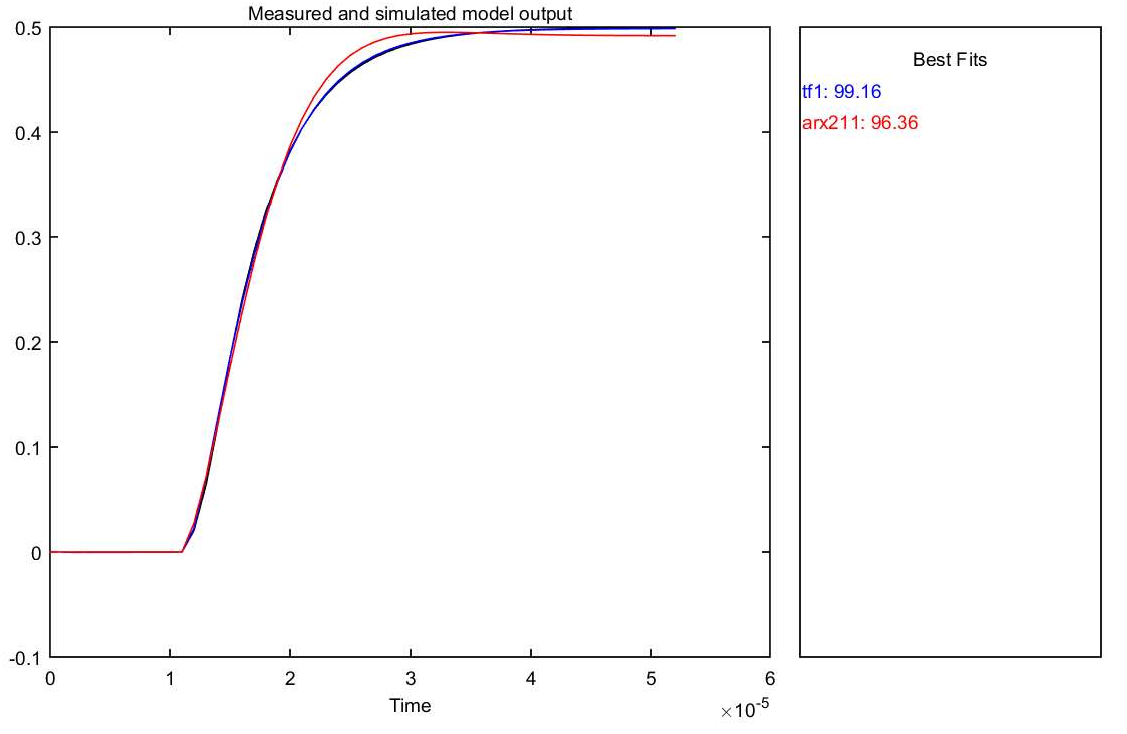
\includegraphics[width = 0.7\textwidth]{assets/image/ESTIMATION MODEL.pdf}
                    \caption{Plot performansi metode estimasi ARX dengan transfer function}
                    \label{fig:my_label}
            \end{figure}
            
            dst ....................................................
            
        \subsection{Pemodelan state space pada sistem mekanik sederhana}
            \begin{figure}[H]
                \centering
                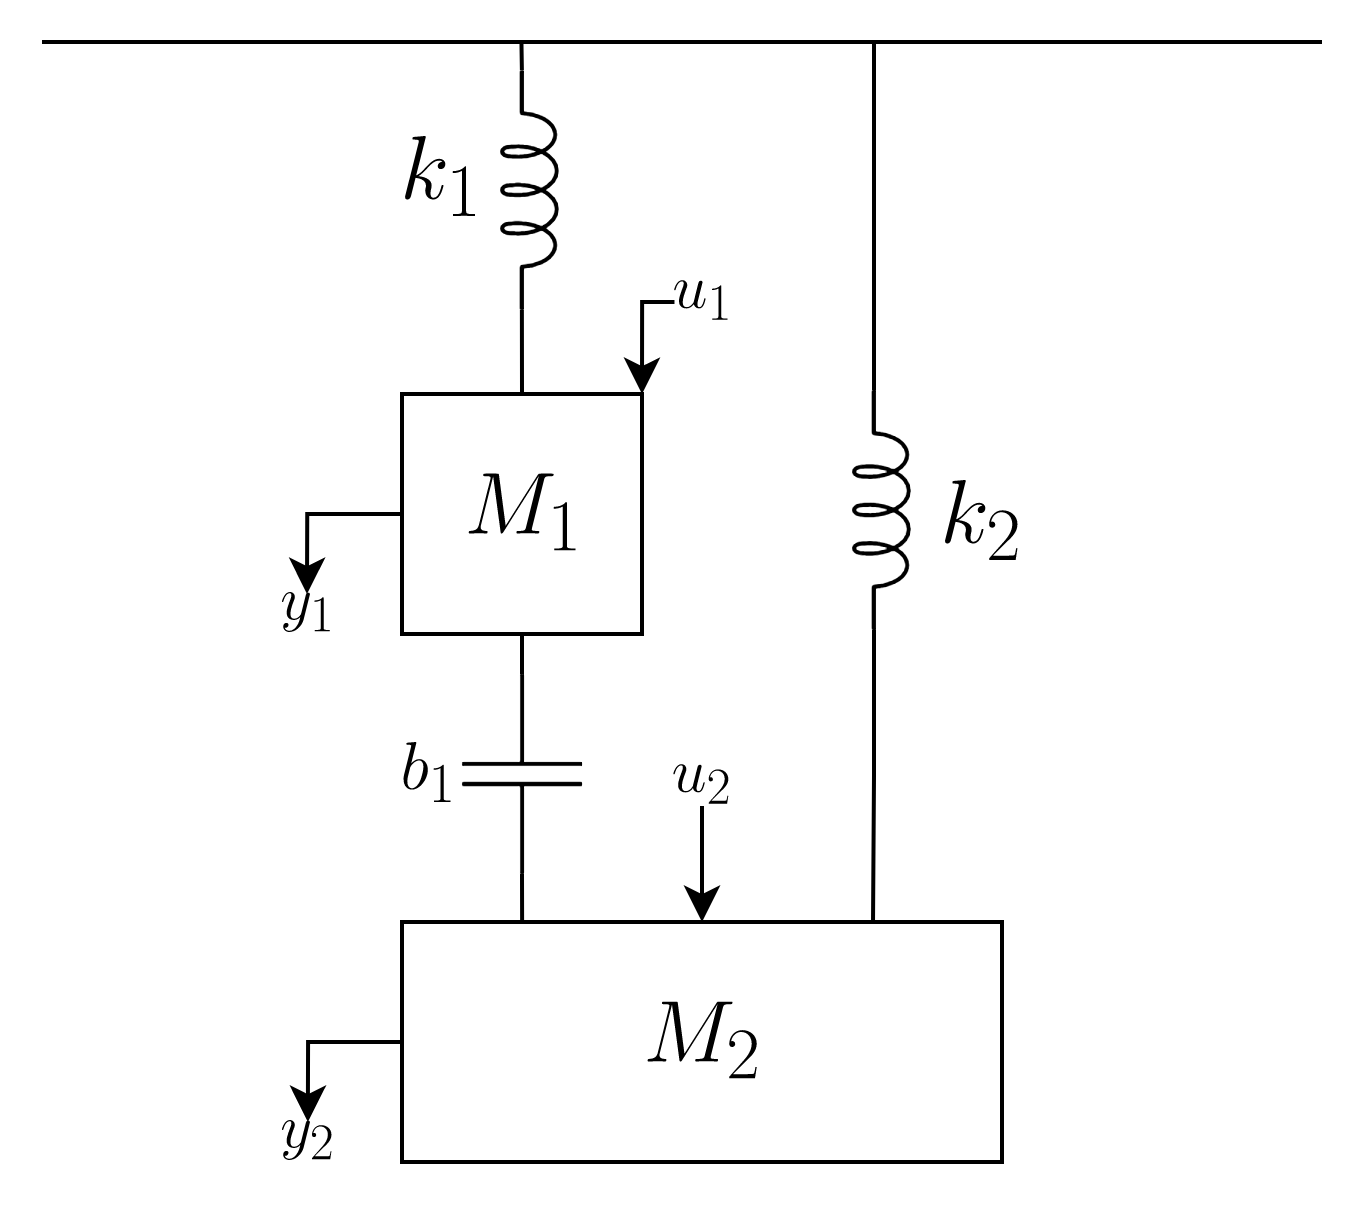
\includegraphics[width = 0.5\textwidth]{assets/image/soal_pemodelan_pegas_damper.png}
                \caption{Model mekanik beban yang digantungkan pada pegas dan damper}
                \label{gambar_4}
            \end{figure}
            dst ....................................................
            
           
        \subsection{Mengubah representasi sistem state space ke fungsi alih}
            \subsubsection{Analisis perubahan representasi state space ke fungsi alih secara matematis}
                \begin{equation}
                    \begin{split}
                        \dot{x} &= Ax + Bu \\[5pt]
                        \begin{bmatrix} \dot{x_1} \\ \dot{x_2} \\ \dot{3} \end{bmatrix} &= \begin{bmatrix} 0 & 1 & 0 \\ 0 & 0 & 1 \\ -2 & -4 & -6 \end{bmatrix} \begin{bmatrix} x_1 \\ x_2 \\ x_3  \end{bmatrix} + \begin{bmatrix} 0 & 0 \\ 0 & 1 \\ 1 & 0 \end{bmatrix} \begin{bmatrix} u_1 \\ u_2 \end{bmatrix} \\[10pt]
                        y &= Cx + Du \\[5pt]
                        \begin{bmatrix} y_1 \\ y_2 \end{bmatrix} &= \begin{bmatrix} 1 & 0 & 0 \\ 0 & 1 & 0 \end{bmatrix} \begin{bmatrix} x_1 \\ x_2 \\ x_3 \end{bmatrix}
                    \end{split}
                \end{equation}

                \begin{equation}
                	\begin{split}
                		\frac{y}{u} &= \frac{10s+10}{s^3+6s^2+5s+10} \\[5pt]
                		\frac{y}{u} &= \underbrace{\frac{1}{s^3+6s^2+5s+10}}_\text{mencari persamaan $\dot{x}=Ax+Bu$} \overbrace{(10s+10)}^\text{mencari persamaan $y=Cx+Du$}
                	\end{split}
               \end{equation}
                
                dst ....................................................
                
                
   		\subsubsection{Analisis perubahan model state space ke fungsi alih dengan MATLAB}
                \lstinputlisting[language = Matlab]{assets/code/SS2TF.m}
            Output program pada konsole MATLAB sebagai berikut,
                \lstinputlisting[]{assets/code/output_SS2TF.m}
            Dari output konsole MATLAB dapat diliha bahwa analisis secara matematis dan analisis dengan MATLAB memiliki hasil yang sama.
            
            
    \section{Kesimpulan}
        Dari hasil dan pembahasan diatas, didapat beberapa kesimpulan sebagai berikut,
        \begin{enumerate}
            \item konversi pemodelan state space ke pemodelan fungsi alih dapat dilakukan dengan persamaan $G_{(s)} = C(sI - A)^{-1} B$
            \item konversi pemodelan sistem dari state space ke pemodelan fungsi alih pada MATLAB dilakukan dengan \textit{system identification toolbox}
        \end{enumerate}
        
        dst ....................................................
        
        
        \bibliographystyle{IEEEtran}
        \bibliography{references}   
    
\end{document}